\section{System analysis}

This chapter presents a systematic analysis of the problem domain, following established system analysis principles.

\subsection{System representation}

The system under study can be represented as a ``black box'' with clearly defined inputs and outputs.
The inputs include raw data, configuration parameters, and user requirements.
The outputs include processed results, performance metrics, and generated reports.

% === EXAMPLE: TikZ black-box diagram with labeled I/O ===
\begin{figure}[H]
    \centering
    \begin{tikzpicture}[
        box/.style={rectangle, draw, thick, minimum width=4cm, minimum height=2.5cm, align=center, fill=gray!10},
        io/.style={->, >=Stealth, thick},
        lbl/.style={font=\small}
    ]
        \node[box] (sys) {\textbf{System}};

        % Inputs
        \node[lbl, left=2.5cm of sys, yshift=0.7cm] (in1) {Raw data};
        \node[lbl, left=2.5cm of sys] (in2) {Configuration};
        \node[lbl, left=2.5cm of sys, yshift=-0.7cm] (in3) {User requirements};

        % Outputs
        \node[lbl, right=2.5cm of sys, yshift=0.5cm] (out1) {Processed results};
        \node[lbl, right=2.5cm of sys, yshift=-0.5cm] (out2) {Performance metrics};

        \draw[io] (in1) -- (sys.west |- in1);
        \draw[io] (in2) -- (sys.west |- in2);
        \draw[io] (in3) -- (sys.west |- in3);
        \draw[io] (sys.east |- out1) -- (out1);
        \draw[io] (sys.east |- out2) -- (out2);
    \end{tikzpicture}
    \caption{System ``black box'' representation} \label{fig:blackbox}
\end{figure}

\subsection{System functions}

The system performs the following primary functions:
\begin{itemize}
  \item data ingestion and preprocessing;
  \item analysis and transformation;
  \item result generation and visualization;
  \item logging and monitoring;
  \item reporting and export.
\end{itemize}

\subsection{System decomposition}

The system is decomposed into four subsystems:
\begin{itemize}
  \item data processing subsystem;
  \item analysis engine subsystem;
  \item user interface subsystem;
  \item monitoring and logging subsystem.
\end{itemize}

\begin{figure}[H]
    \centering
    \begin{tikzpicture}[
        box/.style={rectangle, draw, minimum width=3cm, minimum height=0.8cm, align=center},
        >=Stealth
    ]
        \node[box] (sys) {System};
        \node[box, below left=1cm and 0.5cm of sys] (dp) {Data Processing};
        \node[box, below=1cm of sys] (ae) {Analysis Engine};
        \node[box, below right=1cm and 0.5cm of sys] (ui) {User Interface};
        \node[box, below=1cm of ae] (ml) {Monitoring \& Logging};
        \draw[->] (sys) -- (dp);
        \draw[->] (sys) -- (ae);
        \draw[->] (sys) -- (ui);
        \draw[->] (ae) -- (ml);
    \end{tikzpicture}
    \caption{System decomposition diagram} \label{fig:decomposition}
\end{figure}

\subsection{Hierarchical structure}

The hierarchical organization follows the principle of separation of concerns.
At the top level, the orchestrator manages the overall workflow.
The middle layer contains domain-specific processing modules.
The bottom layer handles infrastructure concerns such as data storage and network communication.

\begin{figure}[H]
    \centering
    \begin{tikzpicture}[
        box/.style={rectangle, draw, minimum width=2.5cm, minimum height=0.7cm, align=center},
        >=Stealth
    ]
        \node[box] (orch) {Orchestrator};
        \node[box, below left=0.8cm and 1cm of orch] (proc) {Processing};
        \node[box, below right=0.8cm and 1cm of orch] (report) {Reporting};
        \node[box, below left=0.8cm and 0cm of proc] (store) {Storage};
        \node[box, below right=0.8cm and 0cm of proc] (net) {Network};
        \draw[->] (orch) -- (proc);
        \draw[->] (orch) -- (report);
        \draw[->] (proc) -- (store);
        \draw[->] (proc) -- (net);
    \end{tikzpicture}
    \caption{System hierarchy diagram} \label{fig:hierarchy}
\end{figure}

\subsection{State machine}

% === EXAMPLE: TikZ state machine / automaton ===
Figure~\ref{fig:state-machine} shows the state transitions of the data processing pipeline.

\begin{figure}[H]
    \centering
    \begin{tikzpicture}[
        state/.style={circle, draw, minimum size=1.5cm, align=center, font=\small},
        accept/.style={state, double},
        >=Stealth,
        auto
    ]
        \node[state] (idle) {Idle};
        \node[state, right=2cm of idle] (load) {Loading};
        \node[state, right=2cm of load] (proc) {Processing};
        \node[accept, right=2cm of proc] (done) {Done};
        \node[state, below=1.5cm of proc] (err) {Error};

        \draw[->] (idle) edge node {\small start} (load);
        \draw[->] (load) edge node {\small data ready} (proc);
        \draw[->] (proc) edge node {\small complete} (done);
        \draw[->] (load) edge[bend right] node[left] {\small fail} (err);
        \draw[->] (proc) edge node[right] {\small fail} (err);
        \draw[->] (err) edge[bend right=50] node[below] {\small retry} (idle);
        \draw[->] (done) edge[bend left=60] node[above] {\small reset} (idle);
    \end{tikzpicture}
    \caption{Processing pipeline state machine} \label{fig:state-machine}
\end{figure}

\subsection{Pie chart of resource allocation}

% === EXAMPLE: TikZ pie chart (manual) ===
The resource allocation across subsystems is shown in Figure~\ref{fig:pie-chart}.

\begin{figure}[H]
    \centering
    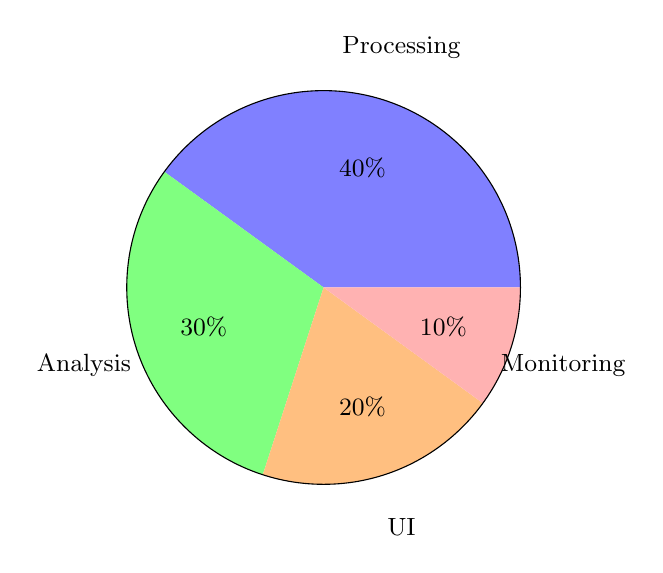
\begin{tikzpicture}
        % Data: Processing 40%, Analysis 30%, UI 20%, Monitoring 10%
        \def\radius{2.5}

        % Processing: 0 to 144 degrees (40%)
        \fill[blue!50] (0,0) -- (0:\radius) arc (0:144:\radius) -- cycle;
        \node at (72:1.6) {\small 40\%};
        \node at (72:3.2) {\small Processing};

        % Analysis: 144 to 252 degrees (30%)
        \fill[green!50] (0,0) -- (144:\radius) arc (144:252:\radius) -- cycle;
        \node at (198:1.6) {\small 30\%};
        \node at (198:3.2) {\small Analysis};

        % UI: 252 to 324 degrees (20%)
        \fill[orange!50] (0,0) -- (252:\radius) arc (252:324:\radius) -- cycle;
        \node at (288:1.6) {\small 20\%};
        \node at (288:3.2) {\small UI};

        % Monitoring: 324 to 360 degrees (10%)
        \fill[red!30] (0,0) -- (324:\radius) arc (324:360:\radius) -- cycle;
        \node at (342:1.6) {\small 10\%};
        \node at (342:3.2) {\small Monitoring};

        % Circle border
        \draw (0,0) circle (\radius);
    \end{tikzpicture}
    \caption{Resource allocation across subsystems} \label{fig:pie-chart}
\end{figure}

\subsection{Summary}

The system analysis reveals that a modular architecture with clear boundaries between subsystems provides the best foundation for achieving the research objectives.

\clearpage
